In order to evaluate both models, the sklearn ``metrics'' library was used, in
particular, the ``classification\_report'', and ``confusion\_matrix'' functions.
The classification reports, shown in Figures \ref{fig:bayesReport} and
\ref{fig:sgdReport} show the Precision, Recall, and F1 Score of each of the
``best case'' models, as described in the preceding section.

\begin{figure}[H]
	\centering
	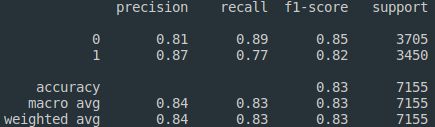
\includegraphics[width=0.8\textwidth]{images/bayesMetricReport}
	\caption{Metrics Report for the Bayes Model}
	\label{fig:bayesReport}
\end{figure}

Precision is defined as the models ability to minimize false positives, i.e.
only label positive data as positive data\cite{skMetric}. As can be seen in the
metrics report for the Bayes model, the precision for ``fake'' articles is
87\%, while the precision for the ``real'' articles is 81\%. Comparing this to
the SGD Model, it can be seen that the precision for ``real'' articles was much
higher in the case of the SGD Model, however there is a much lower value for
precision for the ``fake'' articles.

Recall is defined as the models ability to find all positive
matches\cite{skMetric}. Within the Bayes model, the recall for the ``real''
articles is 89\%, while for ``fake'' articles there is a value of 77\%.
Comparing with the SGD Model, there is a value of only 69\% for the ``real''
articles, with a value of 90\%  for the ``fake'' articles.

Finally, the F score is a weighted average of the precision and recall values.
The Bayes has an F score of 85\% for the ``real'' articles, with a value of 82\%
for the ``fake articles''. The SGD Model has a value of 77\% for the ``real''
articles, with a value of 80\% for the fake articles.

\begin{figure}[H]
	\centering
	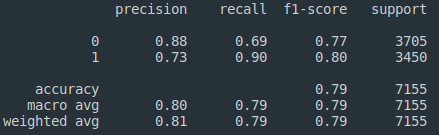
\includegraphics[width=0.8\textwidth]{images/sgdMetricReport}
	\caption{Metrics Report for the SGD Model}
	\label{fig:sgdReport}
\end{figure}

From these classification reports, it is clear that the Bayes classifier is
superior for this classification task. It has a better average precision and
recall for both article types. While the SGD classifier had better precision for
``real'' articles, and better recall for ``fake'' articles than the Bayes
classifier, the overall performance results in a lower oeverall accurracy.

The confusion matrices, as shown below in figures \ref{fig:bayesConf} and
\ref{fig:sgdConf} confirm the evaluation above. The number of false positives
within the Bayes classifier is much lower than that of the SGD Classifier,
however the number of false negatives within the SGD classifier is much lower
than that of the Bayes classifier. Again, the difference leaves a greater
accuracy for the Bayes classifier, making it a more optimal solution for this
assignment.

\begin{figure}[H]
	\centering
	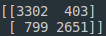
\includegraphics[width=0.8\textwidth]{images/bayesConfMatrix}
	\caption{Confusion Matrix for the Bayes Model}
	\label{fig:bayesConf}
\end{figure}


\begin{figure}[H]
	\centering
	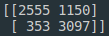
\includegraphics[width=0.8\textwidth]{images/sgdConfMatrix}
	\caption{Confusion Matrix for the SGD Model}
	\label{fig:sgdConf}
\end{figure}
